% ============================================================
% Insurance under Adversarial Risk — journal paper (working title)
% Single-author: Björn Hanneke, Goethe University Frankfurt
%
% Build: latexmk -pdf main.tex   (or use the Makefile / Overleaf)
% Sections live in sections/, proofs in appendix/, figures in figures/
% (regenerated by ../pipeline/dynamic_game/ — see repo README).
% ============================================================
\documentclass[11pt]{article}

\usepackage[margin=1.1in]{geometry}
\usepackage{amsmath}
\usepackage{amssymb}
\usepackage{amsthm}
\usepackage{mathtools}
\usepackage{bm}
\usepackage{booktabs}
\usepackage{graphicx}
\usepackage{setspace}
\usepackage{xcolor}
\usepackage[colorlinks=true,linkcolor=blue!55!black,citecolor=blue!55!black,urlcolor=blue!55!black]{hyperref}
\usepackage[authoryear,round]{natbib}
\usepackage{doi}
\usepackage[capitalise,noabbrev]{cleveref}

% Theorem environments (amsthm)
\theoremstyle{plain}
\newtheorem{theorem}{Theorem}
\newtheorem{proposition}{Proposition}
\newtheorem{lemma}{Lemma}
\newtheorem{corollary}{Corollary}
\theoremstyle{definition}
\newtheorem{definition}{Definition}
\newtheorem{assumption}{Assumption}
\theoremstyle{remark}
\newtheorem{remark}{Remark}

% Operators
\DeclareMathOperator*{\argmax}{arg\,max}
\DeclareMathOperator*{\argmin}{arg\,min}
\DeclareMathOperator{\Var}{Var}
\DeclareMathOperator{\Cov}{Cov}

% Model shorthands (keep in one place so notation stays consistent)
\newcommand{\E}{\mathbb{E}}
\newcommand{\Prob}{\Pr}
\newcommand{\ind}[1]{\mathbf{1}\{#1\}}   % bbm fonts unavailable in tectonic
\newcommand{\Rpos}{\mathbb{R}_+}
\newcommand{\cov}{q}                       % coverage of protocol i: q_i
\newcommand{\poolret}{r^{\mathrm{pool}}}   % pool return schedule
\newcommand{\rmkt}{r^{\mathrm{m}}}         % market rate
\newcommand{\blast}{\beta}                 % extraction (blast-radius) tech
\newcommand{\rent}{\pi}                    % attacker rent


\onehalfspacing

\title{Insurance under Adversarial Risk:\\
Collateral, Deterrence, and the Design of Decentralized Coverage%
\thanks{TODO(BH): acknowledgements, seminar audiences, funding. Working
title --- revise.}}
\author{Bj\"orn Hanneke\\ \small Goethe University Frankfurt}
\date{\today\\ \small Preliminary --- do not cite or circulate.}

\begin{document}
\maketitle

\begin{abstract}
\noindent
% TODO(BH): abstract. Raw material: JournalPaper/positioning_memo.md §1–§2.
% Elements to hit: (i) phenomenon — DeFi exploit losses, uninsurability;
% (ii) the Budish gap: security requires attack cost scaling eta=1, we
% estimate eta ≈ 0.2; (iii) mechanism — coverage pool with negligence-
% contingent collateral forfeiture and a yield carry; (iv) results —
% forfeiture neutralizes attacker-amplified moral hazard (Prop. D
% decoupling), carry is a security subsidy (Prop. C); (v) structural
% calibration on realized hack losses.
\emph{[Abstract to be drafted.]}
\end{abstract}

\bigskip
\noindent\textbf{Keywords:} cyber insurance; decentralized finance;
mechanism design; moral hazard; deterrence; structural calibration.\\
\textbf{JEL:} D82, D86, G22, G23, L86.

\newpage
\section{Introduction}\label{sec:intro}

% TODO(BH): draft. Raw material: JournalPaper/positioning_memo.md §2
% (motivation stack). Suggested skeleton (logic only, prose is yours):
%
% 1. Phenomenon: DeFi exploit losses in the billions annually; smart-
%    contract risk fails classical insurability criteria (Bekemeier 2023);
%    dedicated cover protocols remain marginal; the recognized bottleneck
%    is the yield conundrum (Zhou 2026).
% 2. The tension: insurance under ADVERSARIAL risk. Losses are chosen by
%    a profit-motivated attacker who responds to the contract; evidence
%    that attackers condition on insurance (Meurs et al. 2022: insured
%    victims pay 2.7x larger ransoms; Li & Liao 2025: insurance raises
%    attacker payoffs).
% 3. The Budish gap: incentive-based security requires attack cost
%    scaling ~linearly with value secured (Budish 2025); our structural
%    estimate of the application-layer technology is eta ~ 0.2. The gap
%    between required and actual scaling is the market for insurance.
% 4. This paper: a coverage-pool mechanism whose two DeFi-specific
%    instruments -- negligence-contingent collateral forfeiture and an
%    above-market pool yield -- jointly neutralize attacker-amplified
%    moral hazard. Preview Prop. D (decoupling), Prop. C (carry as
%    security subsidy), and the calibrated counterfactuals (forfeiture
%    off: hacks 2.3 -> 10.8/yr).
% 5. Why blockchain: smart contracts make forfeiture credible and
%    automatic (Corollary D1).

\emph{[To be drafted.]}

\section{Related literature}\label{sec:related}

% TODO(BH): draft from JournalPaper/positioning_memo.md §3 (contribution
% matrix) and §4 (six referee attacks / defense lines). The five papers
% to engage by name, in order:
%
% 1. \citet{bekemeierschar2026}: smart-contract insurance with pooled
%    collateral and parametric payouts -- exogenous loss process; we
%    endogenize the attacker, the security choice, and the forfeiture/
%    carry instruments they hold fixed.
% 2. \citet{liliao2025} (also \citealt{zhaotumu2025}): insurance raises
%    attacker payoffs and collapses security -- the diagnosis; this paper
%    is the mechanism-design and structurally calibrated answer.
% 3. \citet{zhangzhuhayel2017,zhangzhu2020}: attacker-aware contract
%    design via coverage caps -- instruments on the insured's constraint;
%    forfeiture moves the attacker's participation constraint.
% 4. \citet{budish2025}: consensus security requires linear attack-cost
%    scaling; we estimate the application-layer technology (eta ~ 0.2)
%    and design for the shortfall.
% 5. \citet{stakesure2024}: slashed stake as victim compensation -- the
%    forfeited party is the wrongdoer at the consensus layer; here the
%    forfeited party is the insured victim, priced against a strategic
%    attacker in equilibrium.
%
% Secondary positioning: insurance-as-governance without collateral
% (\citealt{benshaharlogue2012,bakergriffith2010,bakershortland2023});
% bonding classics and their critiques
% (\citealt{williamson1983,dickensetal1989}); pre-screening as the
% benchmark cure (\citealt{khalilinaghizadehliu2018}); terrorism
% insurance with a displacing attacker (\citealt{lakdawallazanjani2005});
% the elasticity objects to distinguish: ransom-revenue elasticity ~0.12
% (\citealt{meursetal2023}), victim-loss elasticity 0.23--0.26
% (\citealt{aldasoroetal2022}), white-hat supply 0.1--0.2
% (\citealt{sridharng2021}) -- ours is the attack-COST technology.
% Method pedigree: structural Becker estimation to policy counterfactual
% (\citealt{fuwolpin2018}); quantitative-section template
% (\citealt{mazengzhang2025}); genre precedents
% (\citealt{leharparlour2025,capponijiawang2025,pagnotta2022,
% congetal2025,hasbrouckriverasaleh2026}).

\emph{[To be drafted.]}

\section{Model}\label{sec:model}

% Formal skeleton assembled from pipeline/dynamic_game/PROOF_NOTES.md.
% Connective prose is deliberately minimal and factual; TODO(BH) markers
% flag where argument-carrying prose is to be written.

\subsection{Environment}\label{sec:env}

Time is discrete, $t = 0, 1, \ldots, T$ (quarters). There are $n$
protocols indexed by $i$, protocol $i$ holding value (TVL) $V_{it} > 0$,
and a coverage pool with liquidity-provider (LP) capital $S_t \geq 0$.
Each period, protocol $i$ chooses a security level $h_i \geq 0$ at flow
cost $c_h h_i V_{it}$ and posts collateral $C_i \in [0, \bar{c}\,V_{it}]$
into the pool. Total pool capital is $A_t = S_t + \sum_i C_i$.

\paragraph{Attacker.} A profit-motivated attacker observes
$(V_{it}, h_i)$ and chooses effort $e \geq 0$ per target. Extraction
technology and cost are
\begin{equation}\label{eq:attacker-tech}
  \blast(e, h) = \bigl(1 - e^{-a e}\bigr)(1 + h)^{-\zeta},
  \qquad
  c(e, V) = \bigl(F_0 + \gamma_c e^{\kappa}\bigr) V^{\eta},
\end{equation}
so that a successful exploit extracts $\varepsilon \blast(e,h) V$ with
execution noise $\varepsilon \in [0,1]$,
$\E[\varepsilon] = \bar\varepsilon$. The elasticity $\eta$ of attack cost
with respect to target value is the paper's key structural parameter
(\cref{sec:calibration}); $\kappa$ governs the effort cost curvature.
The attacker's rent against target $(V, h)$ and the induced hack
probability are
\begin{equation}\label{eq:rent}
  \rent(V, h) = \max_{e \geq 0}\;
    \bar\varepsilon\, \blast(e, h)\, V - c(e, V),
  \qquad
  p(V, h) = q \cdot \Bigl(1 - e^{-\rent(V,h)_+ / \bar{F}}\Bigr),
\end{equation}
with $q$ the per-quarter opportunity arrival rate and $\bar{F}$ the
scale of the (smoothed) participation margin. % TODO(BH): footnote on the
% smoothing (heterogeneous outside options) and the exact-threshold variant.

\paragraph{Mechanism.} The pool grants protocol $i$ coverage
\begin{equation}\label{eq:coverage}
  \cov_i = s\,\mu\, C_i^{\theta}\,\bigl(1 + \xi(h_i)\bigr),
  \qquad \theta \in (0,1),
\end{equation}
where $\xi(\cdot)$ is an increasing security kicker and
$s = \min\{1, U_{\max}/U\}$ a prudential cap on utilization
$U = \sum_i \cov_i / A$. Pool capital earns
$\poolret(A) \geq \rmkt$, with either $\poolret$ fixed (baseline) or
declining in pool size toward the market rate,
$\poolret(A) = \rmkt + (\poolret_0 - \rmkt)\,K/(K + A)$ (the
endogenous-$\alpha$ extension). Revenue is split between LPs and
protocols by a utilization- and risk-dependent share $\gamma$;
protocols' share is pro-rata in posted collateral. On a hack with loss
$L_i = \varepsilon \blast V_{it}$, the pool pays the claim
\begin{equation}\label{eq:claim}
  \text{claim}_i = (1 - d)\,\min\{\cov_i,\, L_i\},
\end{equation}
where $d \in [0,1]$ is a coinsurance rate ($d = 0$ in the baseline
mechanism), and --- the design's distinguishing instrument --- the hacked
protocol's collateral $C_i$ is \emph{forfeited} to the pool.
% TODO(BH): institutional paragraph — parametric on-chain trigger, no
% discretionary negligence adjudication; map to MARBLE mechanism Eqs. 2–8.

\paragraph{Protocol payoff.} Protocol $i$'s per-quarter objective is
\begin{equation}\label{eq:protocol-utility}
\begin{aligned}
  U_i(C_i, h_i) ={}& p_i\,\E\bigl[(1-d)\min\{\cov_i, L_i\}\bigr]
     \;-\; p_i\, C_i \,\ind{\text{forfeiture}}
     \;+\; (1 - p_i)\, y_i(C_i) \\
  &- \tfrac{\rmkt}{4} C_i
     \;-\; \tfrac{c_h}{4}\, h_i V_i
     \;-\; p_i \E[L_i]
     \;-\; \rho_i\, p_i\,\bigl(\E[L_i] - \E[\text{claim}_i]\bigr),
\end{aligned}
\end{equation}
where $y_i(C_i)$ is the pro-rata yield share and $\rho_i$ a
protocol-specific loss-aversion weight on uninsured losses.
% TODO(BH): align notation table with MARBLE Eq. (7) and the addon README.

\subsection{Timing and solution concept}\label{sec:timing}

Within each quarter: (1) the mechanism state
$(A, \gamma, s, \text{hazard})$ is quoted; (2) protocols simultaneously
choose $(C_i, h_i)$; (3) the attacker best-responds target-by-target;
(4) hacks realize with noise $\varepsilon$; (5) settlement: claims are
paid, collateral of hacked protocols is forfeited to the pool, LP capital
adjusts, and TVL transitions. % TODO(BH): timing figure (pipeline
% fig_game_structure) and transition equations.

\begin{definition}[Aggregate-taking stage equilibrium]\label{def:ate}
A profile $\{(C_i^*, h_i^*)\}_i$ together with aggregates
$(\gamma^*, s^*, y^*)$ is an aggregate-taking stage equilibrium if
(i) each $(C_i^*, h_i^*)$ maximizes \eqref{eq:protocol-utility} given the
aggregates and the attacker's best response \eqref{eq:rent}, and (ii) the
aggregates are generated by the profile.
\end{definition}

% TODO(BH): remark on epsilon-equilibria in the finite game and the
% continuum limit (existence exact); cite PROOF_NOTES Steps 3 and the
% certification table.

\subsection{Equilibrium existence}\label{sec:existence}

\begin{lemma}[Own-collateral concavity]\label{lem:concavity}
Suppose pool revenue $R(A) = \poolret(A)\,A$ is concave with
$R(0) = 0$. Then protocol $i$'s objective
\eqref{eq:protocol-utility} is concave in own collateral $C_i$ on
$[0, \bar{c} V_i]$ for every fixed $h_i$.
\end{lemma}

\begin{theorem}[Existence]\label{thm:existence}
Under \cref{lem:concavity} and continuity of the aggregate maps, an
aggregate-taking stage equilibrium in pure strategies exists in the
continuous-collateral game with finite security grid; in the
continuum-of-protocols limit an exact equilibrium exists with
$h$ continuous. % TODO(BH/formal): the continuum statement is the target
% theorem for this paper; the finite-grid game admits epsilon-equilibria
% with certified bounds (Appendix~\ref{app:proofs}).
\end{theorem}

\subsection{The carry trade as a security subsidy}\label{sec:carry}

\begin{proposition}[Advantageous selection and carry--security
complementarity]\label{prop:carry}
Let $\chi_i = (1 - p_i)\,\partial y_i/\partial C_i - \rmkt/4 -
p_i \ind{\text{forfeiture}}$ denote the carry margin on posted
collateral. Then (i) $\partial \chi_i / \partial p_i < 0$: safer
protocols earn a strictly higher carry margin, so collateral posting
selects advantageously on security; (ii) with forfeiture on, the cross
partial of $U_i$ in $(C_i, h_i)$ is positive wherever the deterrence
channel $-\partial p_i/\partial h_i\,(\partial y_i/\partial C_i + 1) > 0$
dominates: collateral and security are complements.
\end{proposition}

\subsection{Forfeiture decouples deterrence from indemnity}\label{sec:decoupling}

Let \emph{family A} (indemnity-only contracts) be the set of mechanisms
with forfeiture off and coinsurance $d \in [0,1]$; every classical
indemnity-side instrument (deductible, coinsurance, coverage denial,
negligence exclusion) is a state-contingent choice of $d$. Let
$s(d) \in [0,1]$ be the equilibrium indemnified share of realized losses
and $h^*(d)$ the equilibrium security level.

\begin{lemma}[Indemnity irrelevance to the attacker]\label{lem:irrelevance}
Fix the defender profile $\{(C_i, h_i)\}_i$. The attacker's problem
\eqref{eq:rent} contains no indemnity-side object: $e^*$, $\rent$, and
$p$ are independent of $d$ and of the claim rule. Hence insurance design
affects hack arrivals only through the induced defender choices
$(C_i, h_i)$.
\end{lemma}

\begin{lemma}[The indemnity frontier]\label{lem:frontier}
Within family A, the on-hack utility differential that disciplines
$h_i$ is bounded by the withheld claim,
$\Delta_A \leq \E[\min\{\cov_i, L_i\}]$, so discipline requires
withholding transfer: over the moral-hazard region the attainable set of
family A traces a decreasing frontier $s \mapsto h^*(s)$, and by
\cref{lem:irrelevance} hack intensity increases along it.
\end{lemma}

\begin{proposition}[Decoupling]\label{prop:decoupling}
The forfeiture mechanism ($d = 0$, forfeiture on) attains a
transfer--security pair outside the family-A attainable set:
(i) no indemnity-only contract achieves both the mechanism's indemnified
share and its security level simultaneously; (ii) the mechanism's
equilibrium security strictly exceeds the family-A frontier evaluated at
the mechanism's transfer level. The mechanism does not maximize the
indemnified share itself: concave coverage caps tail claims by design,
so the escape is in the pair, not in either coordinate alone.
(iii) The value of the second instrument is amplified by the strategic
attacker: shutting down the attacker's extensive-margin response
compresses the security gap between the forfeiture mechanism and the
best family-A contract.
% Certified numerically on the calibrated game (strict criteria, PASS):
% frontier Spearman rho = -1.00 (p < 1e-4); at the mechanism's transfer
% share s = 0.876 the interpolated family-A frontier gives h = 0.40
% (~8 hacks/yr); the mechanism delivers h* = 1.15 (the no-insurance
% security level) at 2.1 hacks/yr -- escape gap 0.75 in h. See
% pipeline/dynamic_game/outputs/results_decoupling.json.
% TODO(BH/formal): analytical version for the continuum model --
% supermodularity of the payout term in (-d, h) where coverage binds;
% part (iii) comparative static in d(beta)/dh and the participation
% elasticity via F-bar.
\end{proposition}

\begin{corollary}[Why the hostage is postable]\label{cor:hostage}
The classical objections to forfeitable bonds --- agents cannot or will
not post them, and the bond-holder may seize them opportunistically ---
are answered inside the mechanism: the carry margin
$\chi_i > 0$ (\cref{prop:carry}) compensates the expected forfeiture, and
the parametric on-chain trigger removes adjudicator discretion.
% TODO(BH): connect to Williamson (1983), Dickens et al. (1989) in the
% positioning section; this corollary carries the "why blockchain"
% argument in contract-theoretic form.
\end{corollary}

\section{Structural calibration}\label{sec:calibration}

% TODO(BH): draft. Content plan:
% - The attacker technology c(e,V) = (F0 + gamma_c e^kappa) V^eta with
%   eta ~ 0.20, kappa ~ 2.7 from the companion structural estimation on
%   realized hack losses (FIRM paper -- cite the companion once public).
% - Why these are technology parameters (Lucas-critique robustness of the
%   counterfactuals): eta and kappa describe the exploit production
%   function, not behavior under a particular policy.
% - Distinguish the elasticity objects: this is the attack-COST-vs-target-
%   value elasticity; Meurs et al.'s 0.12 is ransom REVENUE vs victim
%   size; Aldasoro et al.'s 0.23-0.26 is victim LOSS vs firm size.
% - Mechanism-side parameters (mu, theta, yield split, cap policy) from
%   the MARBLE mechanism; population from Pareto TVL; hazard term
%   structure fitted to incident data.
% - Reproduction targets the calibration hits untargeted: ~2.3 hacks/yr,
%   ~56bps loss rate, utilization ~9 (report as a table).
% - Industry contrast: Immunefi prices critical bounties at 10% of TVL
%   (implicit linear scaling) vs the estimated eta ~ 0.2.
% Parameter table: generate from pipeline/dynamic_game/params.py.

\emph{[To be drafted.]}

\section{Quantitative analysis}\label{sec:quant}

% TODO(BH): draft framing. The design counterfactuals (all already
% computed by the pipeline; figures regenerate via
% pipeline/dynamic_game/run_experiments.py, run_extension.py,
% run_deductible_frontier.py):
%
% 1. Attacker-amplified moral hazard: full mechanism vs no-forfeiture vs
%    no-insurance (h* 1.16 -> 0.18; hacks 2.3 -> 10.8/yr).
% 2. The coverage-security frontier and the decoupling escape (Prop. D):
%    fig_decoupling.
% 3. Endogenous pool alpha: carry extinction vs security (capital
%    efficiency frontier in K).
% 4. eta sweep: who is attacked and the system loss rate as the cost
%    technology varies.
% 5. Frontier validation: re-estimating (kappa, eta) from simulated
%    equilibrium incidents (estimator recovers eta with the predicted
%    downward bias).
% TODO(BH): report each counterfactual in percent / dollar terms
% (per positioning_memo.md §5 -- the Ma-Zeng-Zhang configuration).

\begin{figure}[t]
  \centering
  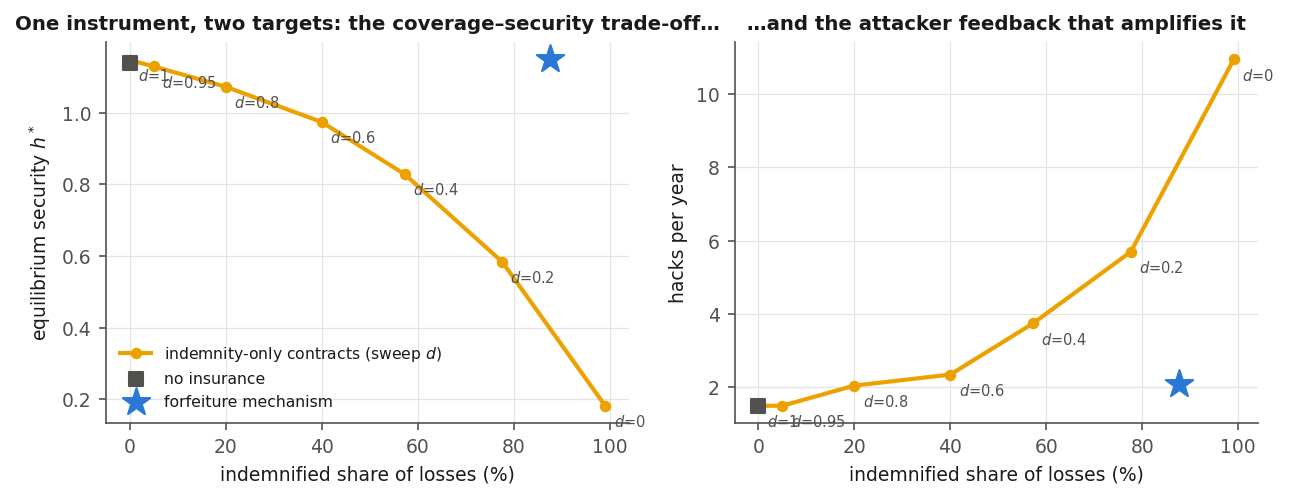
\includegraphics[width=\textwidth]{figures/fig_decoupling.png}
  \caption{The coverage--security frontier of indemnity-only contracts
  (coinsurance $d$ swept from full indemnity to full denial; orange) and
  the forfeiture mechanism (blue star), which attains near-full transfer
  at the no-insurance security level. Left: equilibrium security $h^*$;
  right: realized hack intensity. \emph{[TODO(BH): final caption.]}}
  \label{fig:decoupling}
\end{figure}

\emph{[To be drafted.]}

\section{Design implications and conclusion}\label{sec:design}

% TODO(BH): draft. Candidate content:
% - Pricing/coverage rule implications of eta ~ 0.2 (concave coverage as
%   the answer to whale-targeting).
% - The forfeiture trigger: parametric vs discretionary; seizer-side
%   moral hazard and why the on-chain trigger answers it (Cor. D1).
% - Capital policy: endogenous alpha and the efficiency-security
%   trade-off; what K governs.
% - What traditional carriers can and cannot replicate (the two
%   DeFi-specific instruments).
% - Limitations: finite-grid epsilon-equilibria; single attacker type;
%   no adverse selection on protocol quality beyond TVL; governance risk.

\emph{[To be drafted.]}


\bibliographystyle{plainnat}
\bibliography{references}

\appendix
\section{Proofs and computational certificates}\label{app:proofs}

% Source of record: pipeline/dynamic_game/PROOF_NOTES.md (formal
% development) and pipeline/dynamic_game/prove_equilibrium.py /
% run_deductible_frontier.py (machine certificates). Translate into
% paper-grade proofs here as the stylized (continuum) model firms up.
%
% Inventory to port:
% - Lemma 1 (own-collateral concavity): exact symbolic proof via the
%   A = S + d substitution; 38-monomial numerator, all coefficients
%   nonpositive. -> proof of Lemma \ref{lem:concavity}.
% - Theorem 1' (aggregate-taking existence): Berge + Kakutani on the
%   continuous-collateral game; finite-h-grid caveat and epsilon-Nash
%   certificates (21/24 epochs exact; max eps = $434/quarter).
%   -> proof of Theorem \ref{thm:existence}; continuum limit TODO.
% - Proposition C (carry margin chi, advantageous selection, carry-
%   security complementarity): FOC decomposition; utility-units interior
%   optimality via the stage certificate. -> Prop. \ref{prop:carry}.
% - Lemma A (indemnity irrelevance): by inspection of the attacker's
%   problem. -> Lemma \ref{lem:irrelevance}.
% - Lemma B / Proposition D (frontier + Pareto escape): numerical
%   certification (strict criteria) in results_decoupling.json;
%   analytical continuum version is the open target -- supermodularity
%   of the payout term in (-d, h) where coverage binds.
%   -> Lemma \ref{lem:frontier}, Prop. \ref{prop:decoupling}.
% - Prop. E2'/E3' (carry-trade extinction under endogenous alpha, with
%   the (1-gamma*)C*/S* factor and fee wedge): status INCONCLUSIVE under
%   strict criteria -- decide claim form before submission.

\emph{[Proofs to be ported from the pipeline's proof notes.]}


\end{document}
